\section{Durchführung}
\label{sec:Durchführung}

Der Versuchsaufbau ist in Abb. \ref{fig:aufbau} zu sehen.
\begin{figure}
    \centering
    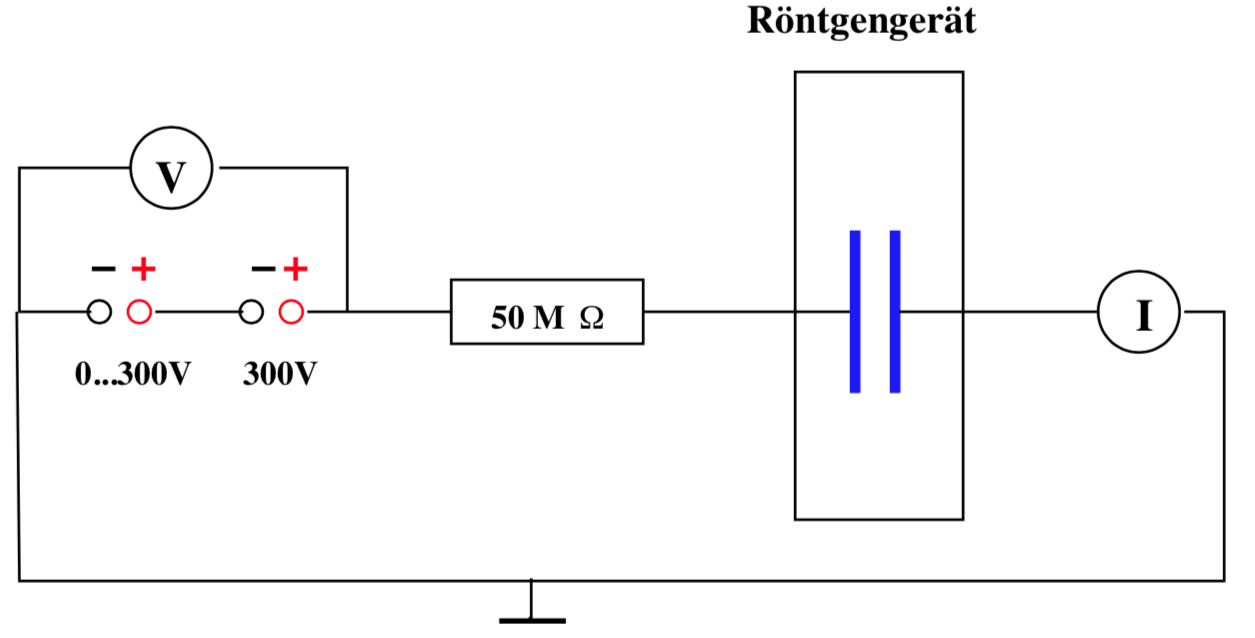
\includegraphics[width=10cm, height=5cm]{build/aufbau.png}
    \caption{Der Versuchsaufbau des Dosimetrie-Versuchs ist hier als Schlatskizze dargestellt. Links gibt es eine Spannungsquelle, in der Mitte befindet sich ein Widerstand, rechts daneben ist ein Röntgengerät eingezeichnet und ganz rechts befindet sich ein Strommessgerät. \cite{V607}}
    \label{fig:aufbau}
\end{figure}

\subsection{Messen der Ionendosisrate j und der Energiedosisrate d}
Die Röntgenröhre wird auf die Beschleunigungsspannung
$U_\text{B} = \SI{25}{\kilo\volt}$ und einen Emissionsstrom 
von $I_\text{A} = \SI{1}{\milli\ampere}$ gestellt.
Es werden die Blenden mit einem Durchmesser von
$d_1 = \SI{2}{\milli\meter}$ und $d_2 = \SI{5}{\milli\meter}$ 
verwendet.
\newline
Der Kondensatorstrom $I_\text{K}$ wird jeweils in Abhängigkeit
von der Kondensatorspannung $U_\text{K}$ in $\SI{50}{\volt}$ 
Schritten gemessen.

\subsection{Messen des Ionenstroms in Abhängigkeit vom Anodenstrom}
Die Röntgenröhre wird wieder auf eine Beschleunigungsspannung von
$U_\text{B} = \SI{25}{\kilo\volt}$ gestellt. Es wird eine
Blende mit dem Durchmesser $d = \SI{5}{\milli\meter}$
verwendet. Die Kondensatorspannung wird auf 
$U_\text{K,1} = \SI{500}{\volt}$ und anschließend auf
$U_\text{K,2} = \SI{300}{\volt}$ eingestellt.
\newline
Es wird jeweils der Kondensatorstrom $I_\text{K}$ in
Abhängigkeit vom Anodenstrom $I_\text{A}$ gemessen.
Der Anodenstrom wird zunächst auf $I_\text{A} = \SI{1}{\milli\ampere}$
gestellt und in $\SI{0.05}{\milli\ampere}$ Schritten verringert.

\subsection{Messen des Ionenstroms in Abhängigkeit von der Beschleunigungsspannung}
Die Röntgenröhre wird auf $I_\text{A} = \SI{1}{\milli\ampere}$
eingestellt. Es wird eine Blende mit $d = \SI{5}{\milli\meter}$
verwendet. Die Kondensatorspannung $U_\text{K,1} = \SI{500}{\volt}$
bzw. $U_\text{K,2} = \SI{300}{\volt}$ wird eingestellt.
\newline
Es wird der Kondensatorstrom $I_\text{K}$ in Abhängigkeit von
der Beschleunigungsspannung $U_\text{B}$ gemessen.
Dabei wird die Beschleunigungsspannung zunächst auf
$U_\text{B} = \SI{35}{\kilo\volt}$ gestellt und anschließend
jeweils um $\SI{5}{\kilo\volt}$ verringert.
